\documentclass{standalone}
\usepackage{pgfplots}
\pgfplotsset{soldot/.style={color=black,only marks,mark=*},
             holdot/.style={color=black,fill=white,only marks,mark=*},
             compat=1.12}
\begin{document}
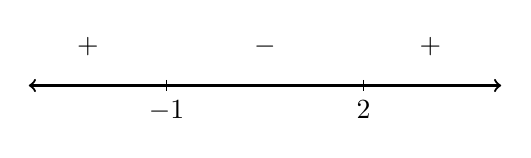
\begin{tikzpicture}
\draw[thick,<->] (-.5,0) -- (5.5,0);
  \draw (1.25 cm,2pt) -- (1.25 cm,-2pt) node[anchor=north] {$-1$};
   \draw (3.75 cm,2pt) -- (3.75 cm,-2pt) node[anchor=north] {$2$};
 \draw (0.25,.5) node {+};
 \draw (2.5,.5) node {$-$};
    \draw (4.6,.5) node {$+$};
\end{tikzpicture}
\end{document}